% Created 2025-01-02 Thu 17:46
% Intended LaTeX compiler: pdflatex
\documentclass[11pt]{article}
\input{../../../preamble.tex}
% setting up title page
\title{
  
\includegraphics[width=0.4\textwidth]{fmf_logo}\\
  {\small Oddelek za fiziko} \\
  {Kotna korelacija anihilicaijskih žarkov $\gamma$}\\
  {\small Poročilo pri FP5}\\
}
\date{}
\author{ Kristofer Č. Povšič, 28211104 \\[5 cm]
 \small  Asistent: Tilen Knaflič \\
}
\begin{document}

\maketitle
\newpage
\tableofcontents

\section{Uvod}\label{sec:org254d4af}

Pozitron \(e^+\) se pri srečanju s svojim antidelcem elektronom \(e^-\) anihilira. Sproščena energija je v obliki elektromagnetnega valovanja.

Zanima nas, ali mogoče nastane pozitronij, vodikovemu atomu podobna tvorba, v kateri elektron in pozitron krožita okoli skupnega težišča.

V osnovnem stanju pozitronija sta si delca najbližje skupaj. Orbitalna vrtilna količina je \(l = 0\). Tako pozitron kot elektron imata spin \(\frac{1}{2}\), zato se osnovno stanje razcepi na singletno stanje z vrtilno količino \(0\) ter tripletno stanje, ki ima vrtilno količino \(1\). Singletno stanje ima vezavno energijo \(6.8 \mathrm{eV}\), medtem ko pa je tripletno za  \(10^{-3} \mathrm{eV}\) manj vezano.

Poglejmo si anihilacijo v singletnem stanju. Predpostavimo, da pozitronij miruje (če ne bi, bi pa obravnavali v CMS in pretvorili v laboratorijski sistem). Ker je vrtilna količina sistema enaka 0, so si v prostoru vse smeri enakovredne. Pri anihilaciji nastali foton torej odleti v katerokoli smer. Zaradi ohranjanja vrtilne količine pa mora nastati še en foton, ki odleti v nasprotno smer. Oba fotona sta ali levo ali desno cirkularno polarizirana.

V tripletnem stanju ne more doseči ohranitve vrtilne in gibalne količine z dvema fotonoma in so potrebni trije.

Bolj pogosto opazimo singletno anihilacijo, navkljub temu da ima tripletno stanje 1000-krat daljšo življenjsko dobo, \(\approx 10^{-7}\), kar tripletu da dovolj časa, da trka z atomi in pri tem preide v singletno stanje.

Pri vaji se uporablja \(^{22} \mathrm{Na}\), ki preko \(\beta^+\) razpada služi kot vir pozitronov. Ta se anihilira z elektronom, pri čemer nastaneta dva kolinearna fotona z energijo \(511 \mathrm{keV}\).
\section{Potrebščine}\label{sec:org9bc5234}

\begin{itemize}
\item \(^{22} \mathrm{Na}\) sevalec
\item 2 scintilacijska detektorja
\item časovno-digitalni pretvornik (ang. \emph{time-to-digital converter} ali TDC) Red Pitaya
\item 2 modula
\item 8 kanalni razdelilec z zakasnilno enoto
\end{itemize}

\section{Naloge}\label{sec:orge32db56}

\begin{itemize}
\item inicializiraj časovno-digitalni pretvornik na plošči Red Pitaya in opravi kalibracijo
\item izmeri ločljivost časovno-digitalnega pretvornika
\item izmeri porazdelitev časovnih intervalov med razpadi radioaktivnega vira
\item poišči koincidence anihilacijskih žarkov \(\gamma\) in izmeri njihovo kotno korelacijo
\end{itemize}

\section{Meritve in izračuni}\label{sec:org032569d}

Na diskriminatorju ORTEC 9302 sem nastavil nivo na vrednost, ki ustreza dolini pod fotovrhom in s tem se izločil ostale signale, ki niso bili pomembni.

Slika na oscilatorju, ko so že nastavili nivo je bila takšna kot na sliki \ref{fig:caspot}

\begin{slika}[H]
  \centering
  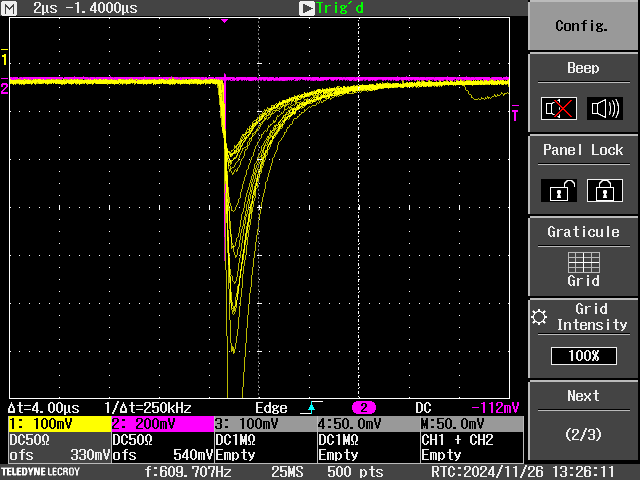
\includegraphics[width=.9\linewidth]{figures/casovni_potek.png}
  \caption{\small Fotografija časovnega poteka, ki je bila videna na oscilatorju.}\label{fig:caspot}
\end{slika}

S pomočjo modula EG\&G-ESN GG8000, ki služi kot oblikovalnik sunkov, zakasnilna enota in razdelilec smo napeljali signal na Red Pitaya.

Na diskriminatorju smo prav tako širino signalov nastavili na približno \(100 \mathrm{ns}\), kar je pomenilo, da signal izgleda tako kot na sliki \ref{fig:prisig}

\begin{slika}[H]
  \centering
  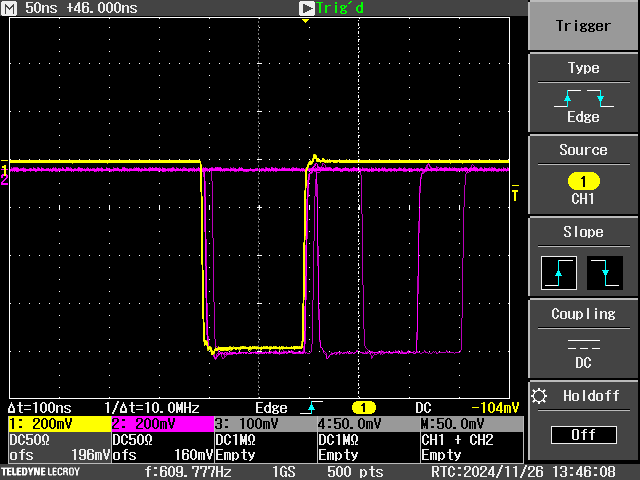
\includegraphics[width=.9\linewidth]{figures/pripravljen_signal.png}
  \caption{\small Fotografija pripravljenega signala kot je bila videti na oscilatorju.}\label{fig:prisig}
\end{slika}

\subsection{Časovna ločljivost TDC}\label{sec:org81fd923}

Pri merjenju časovne ločljivosti je na oba kanala pretvornika poslan isti signal in pričakovali bi, da je ob vsakem sunku izmerjen identični časovni interval. V praksi so izmerki razstreseni okoli povprečja ločljivosti TDCja.

Oblika časovne ločljivosti je Gaussova krivulja in se jo vidi na sliki \ref{fig:casloc}. Lastnosti Gaussove krivuljo so bili

\begin{align*}
x_{0RP} &= 4.59 \mathrm{ps} \\
\sigma_{RP} &= 20 \mathrm{ps}
\end{align*}

Iz zanimanja sem narisal še svojo Gaussovo krivuljo na podatke in dobil sledeče vrednosti

\begin{align*}
x_{0fit} &= (2.6 \pm 0.7) \mathrm{ps} \\
\sigma_{fit} &= (19.6 \pm 0.7) \mathrm{ps}
\end{align*}

Vidimo, da se moja regresija približno ujema s podatki iz RedPitayje.

\begin{slika}[H]
  \centering
  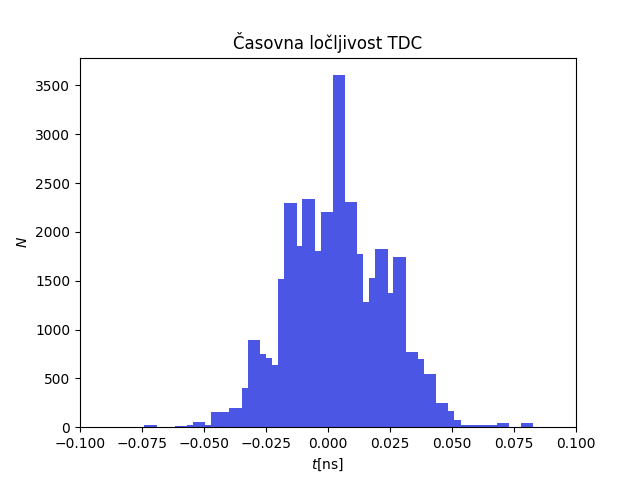
\includegraphics[width=.9\linewidth]{figures/casovna_locljivost.png}
  \caption{\small Graf prikazuje časovno ločljivost grafa. Kot pričakovano je oblike Gaussove krivulje.}\label{fig:casloc}
\end{slika}

\subsection{Radioaktivni razpad}\label{sec:orgb5a1d2e}

Sedaj sem priklopil vsak kanal na svoj scintilacijski detektor in zanimala nas je naključna narava radioaktivne razpada, ki velja za Poissonov proces. Meritev sem opravljal \(t = 31.5 \mathrm{s}\).

Verjetnost, da zaznamo razpad pada eksponentno s časom \(t\)

\begin{equation}
\label{eq:1}
p = 1 - e^{-Rt}
\end{equation}

\begin{slika}[H]
  \centering
  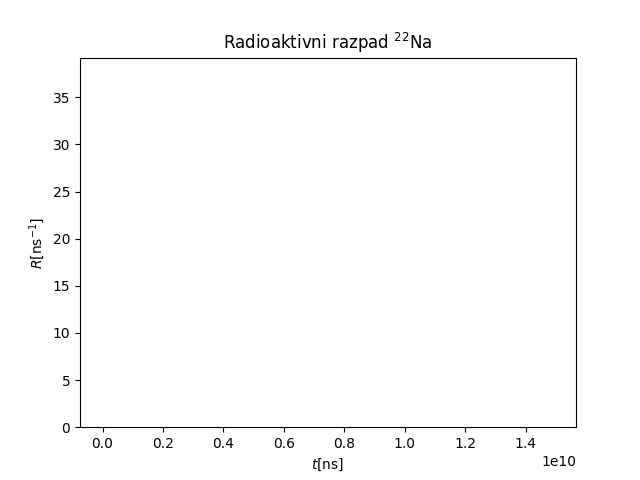
\includegraphics[width=.9\linewidth]{figures/radio_razpad.png}
  \caption{\small Graf prikazuje radioaktivni razpad $^{22} \mathrm{Na}$, ki je po pričakovanjih Poissonove oblike.}\label{fig:radraz}
\end{slika}

Verjetnostno gostoto dobimo z odvajanjem po času, kar nam po logaritmiranju da

\begin{equation}
\label{eq:2}
\ln \left( \frac{\mathrm{d} p}{\mathrm{dt}} \right) = \ln R - Rt
\end{equation}

\begin{slika}[H]
  \centering
  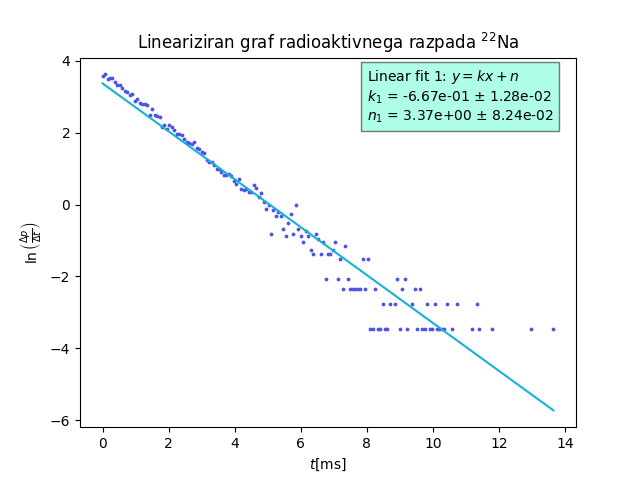
\includegraphics[width=.9\linewidth]{figures/log_radio_razpad.png}
  \caption{\small Graf prikazuje logaritmirane vrednosti grafa \ref{fig:radraz}. S tem smo potrdili, da je porazdelitev res eksponentna.}\label{fig:logradraz}
\end{slika}

Z logaritmiranjem vrednosti smo dobili potrditev, da je porazdelitev zares eksponenta.

Prav tako je vrednost iz logaritmiranja premice enaka

\[ R = (667 \pm 13) \mathrm{s}^{-1}
\]

\subsection{Kotna korelacija anihilacijskih žarkov $\gamma$}\label{sec:orgbb3588f}

S scintilatorskima detektorjema na isti premici sem najprej izmeril meritev koincidenčnih žarkov. Ko se elektron in pozitron anihilirata nastaneta \(\gamma\) žarka v nasprotnih smereh. Če v nekem časovnem obdobju zaznamo sunek toka na obeh scintilatorjih, to smatramo kot koincidenco.

Dobim graf na sliki \ref{fig:koivrh}

\begin{slika}[H]
  \centering
  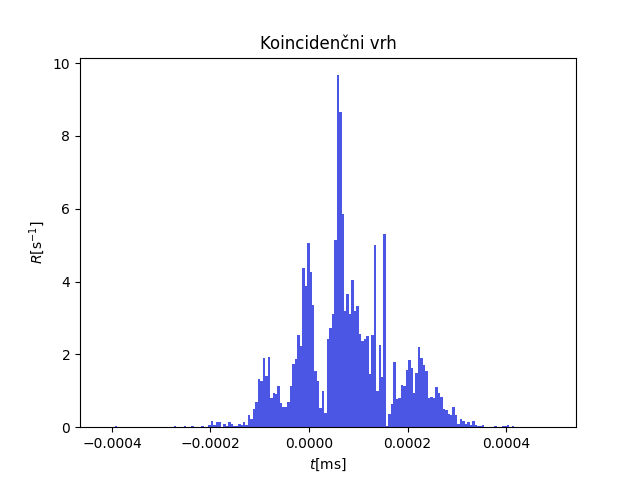
\includegraphics[width=.9\linewidth]{figures/koincidencni_vrh.png}
  \caption{\small Graf prikazuje koincidenčni vrh pri kotu $0^{\circ}$}\label{fig:koivrh}
\end{slika}

Zanimajo nas tudi naključne koincidence. Če je hitrost sunkov na prvem kanalu \(R_1\) in na drugem kanalu \(R_2\) in je širina merilnega okna \(\tau\), potem je hitrost naključnih koincidenc enaka

\begin{equation}
\label{eq:3}
R_{12} = \tau R_1 R_2
\end{equation}

\begin{slika}[H]
  \centering
  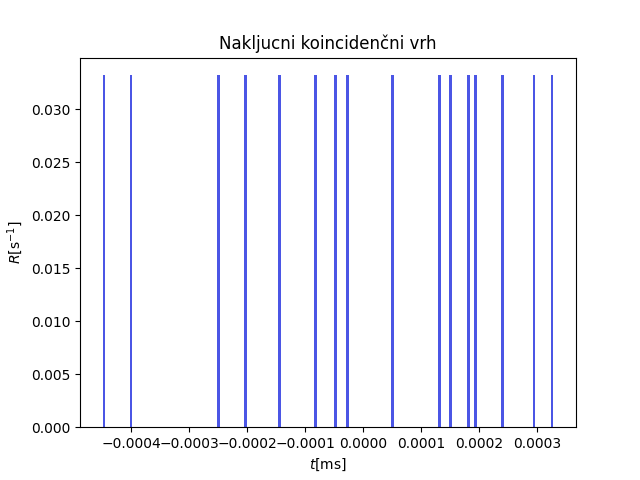
\includegraphics[width=.9\linewidth]{figures/nakljucne_koincidence.png}
  \caption{\small Graf prikazuje naključne koincidence}
\end{slika}

\begin{slika}[H]
  \centering
  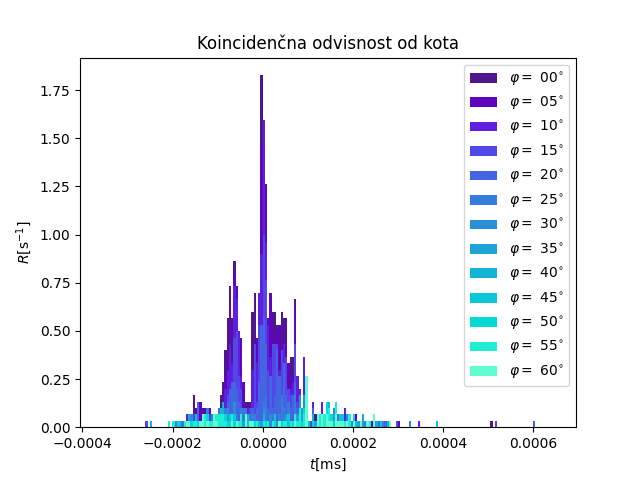
\includegraphics[width=.9\linewidth]{figures/koincidence_kot.png}
  \caption{\small Graf prikazuje odvisnost koincidence od kota med scintilatorskima detektorjema.}\label{fig:test}
\end{slika}

Za zadnji del vaje sem izmeril še kotno korelacijo žarkov z zamikanjem enega od scintilacijskih detektorjev. Meril sem v intervalu \(\varphi = [0, \frac{\pi}{3}]\), kjer je interval med vsako meritvijo 5. Izkaže se, da je število koincidenc močno odvisno od kota, kar se tudi pozna na grafu %\ref{fig:test}.

\section{Komentar}\label{sec:org1a6bddf}

Sama izvedba vaje je predstavljala problem, saj sem se zaradi nepoznavanja naprav precej lovil. Prav tako je bilo potrebno RedPitayjo večkrat ponovno ugasniti in znova prižgati.
Vaja je bila v splošnem uspešna. Uspeli smo določiti časovno ločljivost TDCja, potrdili naključno naravo radioaktivnega razpada, opazovali naključne koincidence ter odvisnost koincidenčnega vrhu v odvisnost od kota med scintilatorjema.

\end{document}
